% thesis.tex
%
% This file is root file for an example thesis written using the
% IIT Bombay LaTeX Style file.
% Created by Amey Karkare (21 June 2007)
%
% It is provided without warranty on an AS IS basis.

%=====================================================================
% Read: http://www.cse.iitb.ac.in/karkare/iitbthesis/
%    FAQ.txt     for frequently asked quetions
%    Changes.txt for changes
%    README      for more information
%=====================================================================

%=====================================================================
% DOCUMENT STYLE
%=====================================================================
% IITB PhD Thesis format default settings are:
%   12pt, one-sided printing on a4 size paper
\documentclass[openright,twoside]{iitkthesis}
% For two-sided printing, with Chapter starting on odd-numbered pages,
% use the following line instead:
%%\documentclass[openright,twoside]{iitbthesis}

%=====================================================================
% OPTIONAL PACKAGES
%=====================================================================
% To include optional packages, use the \usepackage command.
% For e.g., The package epsfig is used to bring in the Encapsulated
%    PostScript figures into the document.
%    The package times is used to change the fonts to Times Roman;
%=====================================================================

%=====================================================================
%  Single counter for theorems and theorem-like environments:
%=====================================================================
\newtheorem{theorem}{Theorem}[chapter]
\newtheorem{assertion}[theorem]{Assertion}
\newtheorem{claim}[theorem]{Claim}
\newtheorem{conjecture}[theorem]{Conjecture}
\newtheorem{corollary}[theorem]{Corollary}
\newtheorem{definition}[theorem]{Definition}
\newtheorem{example}[theorem]{Example}
\newtheorem{figger}[theorem]{Figure}
\newtheorem{lemma}[theorem]{Lemma}
\newtheorem{prop}[theorem]{Proposition}
\newtheorem{remark}[theorem]{Remark}

\usepackage{minted}
\usemintedstyle{bw}

\usepackage{fontspec}
\setmonofont[Scale=0.85]{DejaVu Sans Mono}

\usepackage[sorting=none, maxbibnames=99, minbibnames=99]{biblatex}
\bibliography{citations}
\usepackage{amsmath}
\usepackage{lipsum}
\usepackage{float}
\usepackage[hidelinks]{hyperref}
\usepackage{microtype}
\usepackage[font=small,labelfont=bf]{caption}
\usepackage{fancyref}
\usepackage{color,soul} % for highlights
\usepackage{enumerate}
\usepackage{tabularx}

\setlength{\headheight}{15pt}

\expandafter\def\csname PY@tok@err\endcsname{}

\floatstyle{ruled}
\newfloat{program}{thp}{lop}
\floatname{program}{Figure}

\numberwithin{program}{chapter}

\BeforeBeginEnvironment{program}{\begin{singlespace}}
\AfterEndEnvironment{program}{\end{singlespace}}

%=====================================================================
% End of Preamble, start of document
%

\begin{document}

%=====================================================================
% Include the prelude for Title page, abstract, table of contents, etc
% You need to modify it to contain your details
% prelude.tex
%   - titlepage
%   - dedication (optional)
%   - approval sheet
%   - course certificate
%   - table of contents, list of tables and list of figures
%   - nomenclature
%   - abstract
%============================================================================


\clearpage\pagenumbering{roman}  % This makes the page numbers Roman (i, ii, etc)



% TITLE PAGE
%   - define \title{} \author{} \date{}
\title{Hot Code Reloading in Cloud Haskell (tentative)}
\author{Pankaj More}
\date{June, 2014}

%  - Roll number, required for title page, approval sheet, and
%    certificate of course work
\rollnum{Y9227402}

%   - The default degree is ``Doctor of Philosophy''
%     (unless the document style msthesis is specified
%      and then the default degree is ``Master of Science'')
%     Degree can be changed using the command \iitbdegree{}
\iitbdegree{Master of Technology}

%   - The default report type is preliminary report.
%      * for a PhD thesis, specify \thesis
\thesis
%      * for a M.Tech./M.Phil./M.Des./M.S. dissertation, specify \dissertation
%\dissertation
%      * for a DIIT/B.Tech./M.Sc.project report, specify \project
%\project
%      * for any other type, use  \reporttype{}
%\reporttype{ReportType}

%   - The default department is ``Unknown Department''
%     The department can be changed using the command \department{}
\department{Computer Science \& Engineering}

%    - Set the guide's name
\setguide{Prof Amey Karkare}
\setguidedept{Department of Computer Science \& Engineering}

%   - once the above are defined, use \maketitle to generate the titlepage
\maketitle

%--------------------------------------------------------------------%
% CERTIFICATE
%     The first page after the title page.
\makecertificate

%--------------------------------------------------------------------%
% COPYRIGHT PAGE
%   - To include a copyright page use \copyrightpage
% \copyrightpage

%--------------------------------------------------------------------%
% ABSTRACT
\begin{abstract}
TODO : Abstract
\end{abstract}

%--------------------------------------------------------------------%
% DEDICATION
%   Dedications, if any.
\begin{dedication}
To my grandfather
\end{dedication}

% Acknowledgements
\begin{acknowledgments}

TODO : ACK
% This project would have never have even been started had it not been for my
% thesis advisor Dr Amey Karkare's help and guidance. Right from the time we
% were looking for ideas to when we finally had a concrete proposal in hand, his
% support has been invaluable. He entertained all my crazy ideas, found which
% ones had merit, and helped me build on them. I wouldn't have been able to do
% this without him.

% I'd like to thank my parents and the others in my life for being patient with
% me, especially towards the final stretch of thesis completion when I wasn't at
% my best socially.

% The Racket community, at \texttt{\#racket} on Freenode IRC, helped me
% understand some of the Racket syntax model's intricacies. That helped me avoid
% dead ends both early on and towards the end.

% Special thanks to Leonardo de Moura at Microsoft Research for taking the time
% out to answer a few questions about Z3.

\end{acknowledgments}

%--------------------------------------------------------------------%
% CONTENTS, TABLES, FIGURES
\tableofcontents
\listoftables

\cleardoublepage
\phantomsection \label{listoffig}
\addcontentsline{toc}{chapter}{List of Figures}
%\listof{program}{List of Figures}
%\listoffigures

\cleardoublepage\pagenumbering{arabic} % Make the page numbers Arabic (1, 2, etc)


%=====================================================================
% Include the technical part of the report
%% \include{chap_intro}             % Chapter 1: Introduction
%% \include{chap_others}            % Other chapters as required
%% \include{chap_conclusions}       % Finally the summary & conclusions

%=====================================================================
% APPENDIX
%  Appendices, if any, must precede the cited literatures.
%  Appendices shall be numbered in Roman Capitals (e.g. Appendix IV)

%% \appendix
%% \include{appendix_something}

%=====================================================================
% PUBLICATIONS
%  publications if any may be listed after the literature cited.
%% \include{mypubs}

%=====================================================================
% ACKNOWLEDGMENTS
%   This is the last item in the thesis. It should be signed by
%   author, with date.


\chapter{Introduction}
\label{chap:intro}

With CPU speeds stagnating, the standard approach for increasing performance
is by using more CPUs rather than faster CPUs.  The cost of scaling
the number of cores on a multi-core CPU is quite prohibitive and
renders the model of vertical scaling both inflexible and inelastic
for a range of real-world applications. Horizontally scaling the
computation across a range of commodity compute nodes is much more
cost effective, scales more incrementally and is becoming increasingly
popular for programming compute intensive distributed applications. We
refer to this approach of renting a cluster of nodes with on-demand
elastic scaling of resources and cost as ``cloud computing''. Cloud
Haskell {cite paper here} is a framework for writing distributed applications in
Haskell.

\section{Challenges in a distributed system}

Developing distributed programs which can scale horizontally across a
large number of clusters presents some unique challenges:

\begin{itemize}
\item When programming the cluster as a whole, there is a need to
  coordinate various processes running on heterogeneous systems. Most
  programming languages do not directly address the problem of
  distributed concurrency. The dominant model of concurrency in most
  mainstream programming languages is usually the shared-memory
  variety. It relies on the concept of multiple threads modifying
  shared mutable data. This model is not very useful in a distributed
  model. HdH {cite} tries to replicate the model of shared memory concurrency
  in a distributed system by using the concept of distributed
  MVars. This model is not very successful because the cost of moving
  data across in a distributed system becomes a dominant factor. By
  making message passing explicit, Cloud Haskell exposes the cost of
  message passing to the programmer.
\item The problem of fault tolerance becomes non-trivial in a
  distributed system. When a distributed program is running across
  hundreds of thousands of nodes, some of the nodes will fail at any
  given moment of time. A failure of a node should not require
  restarting the whole calculation , or it might never finish. The
  programmer needs tools to detect and respond to failures as part of
  the programming model. Cloud Haskell allows monitoring of processes
  and exposes primitives to handle node failures.
\end{itemize}

\section{The Problem of Hot Code Reloading}

\subsection{The Problem}

Current cloud haskell systems cannot be easily upgraded from one
verison of the code to the next. There is no support in the tool to
enable safe upgrades. Moreover, if there are multiple versions running
concurrently, processes having incompatible types won't communicate
and the current implementation fails silently. This makes debugging
very hard since the programmer cannot figure out if no error is
generated for incompatible versions. Ad hoc update mechanisms like
using external tools for updating a cluster are neither safe nor
efficient and simply restart the whole system.

In this thesis, we work on the problem of dynamically updating a
running cloud haskell system with zero downtime.

\subsection{The Motivation}

\begin{itemize}
\item Zero downtime is a fairly common requirement in large scale
  distributed systems running critical business logic. This is
  especially true in financial transaction systems, telephone
  switches, airline traffic control systems and other mission
  critical systems.
\item Hot code reloading is less expensive than using redundant
  hardware for managing upgrades. Loss of web service during
  maintenance is no more acceptable and leads to lost revenues. For
  example, Visa makes use of 21 main frames to run its
  fifty-million-line transaction processing system. It is selectively
  able to take machines down and upgrade them by preserving relevant
  state in other online systems and complex state migration. This
  approach is expensive as well as increases the complexity of
  deploying updates.
\item It helps in rapid prototyping and increases developer
  productivity by reducing the length of an iteration cycle. The
  ability to modify a running program and update it on the fly saves a
  lot of time which would be otherwise wasted in restarting a program
  and rebuilding all the relevant state. Moreover, the real time
  feedback available to the programmer when he changes the program is
  very valuable in supporting interactive programming.
\item Language level updating facility is more reliable than using
  external tools to safely update a software. Manually distributing
  the updated version using tools like scp, puts the burden of
  responsibility on the programmer to make sure that all nodes are
  running the same node. This can be quite error-prone because Cloud
  Haskell would silently fail during communication between processes
  of incompatible types.
\end{itemize}

\subsection{Example of Hot Code Reloading in Erlang}

Erlang supports language level dynamic software updating. A process in
erlang can update into the new version by making an external call to
its module.

We demonstrate an example of hot code reloading in erlang by the help
of a counter process. It can receive a message to increment the
running counter, or a message to send the current counter value, it
can also receive a message to update itself.

\begin{program}
\caption[An example of hot code loading]
{Hot code loading in erlang : version 1}
\label{fig:erlang-v1}

\begin{minted}{erlang}
  %% A process whose only job is to keep a counter.
  %% First version
  -module(counter).
  -export([start/0, codeswitch/1]).

  start() -> loop(0).

  loop(Sum) ->
    receive
       {increment, Count} ->
          loop(Sum+Count);
       {counter, Pid} ->
          Pid ! {counter, Sum},
          loop(Sum);
       update ->
          ?MODULE:codeswitch(Sum)
          % Force the use of 'codeswitch/1' from the latest MODULE version
    end.

  codeswitch(Sum) -> loop(Sum).
\end{minted}
\end{program}

In version 2, we add the possibility to reset the counter to 0.

\begin{program}
\caption[An example of hot code loading]
{Hot code loading in erlang : version 2}
\label{fig:erlang-v2}

\begin{minted}{erlang}
 %% Second version
  -module(counter).
  -export([start/0, codeswitch/1]).

  start() -> loop(0).

  loop(Sum) ->
    receive
       {increment, Count} ->
          loop(Sum+Count);
       reset ->
          loop(0);
       {counter, Pid} ->
          Pid ! {counter, Sum},
          loop(Sum);
       update ->
          ?MODULE:codeswitch(Sum)
    end.

  codeswitch(Sum) -> loop(Sum).
\end{minted}
\end{program}

On receiving a ``update'' message, loop will execute an external call
to codeswitch. If there is a new version of ``counter'' module in
memory, the its codeswitch function will be called with the update
state. In our example, we pass the same state to the new version.

The goal of hot code reloading in Cloud Haskell is to have similar
style of code upgrade facility as Erlang.

\section{Performance issues in Cloud Haskell}

While working on the problem of hot code reloading, we came across a
number of performance issues in the current implementation of Cloud
Haskell. Compared to Erlang which has been extensively used in large
scale production systems and extensively improved since last twenty
years, Cloud Haskell was developed only two years back. It has not
been extensively used in production nor any extensive bench-marking
been done with other systems like Erlang. Performance is a major
concern when developing large scale distributed systems which cost a
lot of resources and money.

\section{Our Contributions}

The contributions made in this thesis are:
\begin{itemize}
\item A prototype implementation for upgrading a single cloud haskell
  instance with possibility of intermittent message loss during the
  update.
\item A discussion on other potential approaches to hot code reloading
  in Cloud Haskell like systems.
\item An exhaustive evaluation of the trade-offs in the different
  approaches.
\item Investigation of some performance issues in the current release
  of Cloud Haskell specifically related to the performance of garbage
  collection.
\end{itemize}

The rest of the thesis is organized as follows. Chapter 2 gives a
brief tour of Cloud Haskell and the design decisions taken which set
the background for understanding the rest of the thesis. Chapter 3
highlights the major related work in the field of Dynamic Software
Updating. Chapter 4 describes our approach to hot code reloading in
Cloud Haskell. Chapter 5 briefly talks about the performance issues we
found in Cloud Haskell.
%%% Local Variables:
%%% mode: latex
%%% TeX-master: t
%%% End:

\chapter{A brief tour of Cloud Haskell }
\label{chap:cloudhaskell}

In this chapter, we will briefly cover the overall design decisions
which influence the development of Cloud Haskell. This is really
important in understanding the trade-offs taken by Cloud Haskell. The
problem of hot code reloading and our implementation in the following
chapters depends on the understanding of these decisions.

\section{The Design Decisions}

\subsection{Erlang Style Concurrency}

The key idea is : Program the cluster as a whole, not individual
nodes. Same program runs on all the nodes. The programmer does not
have to worry about how the individual nodes behave. To implement this
model, Cloud Haskell takes inspiration from the Erlang style of
programming which has been highly successful in the industry. The
design decisions are influenced heavily by the motto: ``If in doubt,
do it the way Erlang does it''.  What does Cloud Haskell bring to the
table?
\begin{description}
\item [Improved tooling and library ecosystem] Compared to Erlang,
  Haskell has a much more mature ecosystem of tools and libraries. The
  package manager of Haskell, Hackage has more than 5000 packages
  covering a variety of domains.
\item [Static vs Dynamic Typing] Haskell's static typing with type
  inference eliminates whole class of bugs at compile time.
\item [Modular Architecture] Erlang is the actor model. The networking
  stack is embedded into the run time of Erlang. It is impossible to
  use Erlang in exotic network protocols such as infiniband, CCI, etc
  Cloud Haskell on the other hand keeps the network stack as a library.
\item [Multiple Concurrency Abstractions] Apart from message passing
  across nodes, individual nodes can still use concurrency primitives
  such as Threads and STM as necessary. In case of high capacity,
  multi-core nodes, it might make better sense to use shared
  concurrency constructs than actor model and Cloud Haskell allows
  that. It encourages right abstraction at the right level. Erlang
  does not provide other concurrency primitives.
\item [A more precise and well-defined semantics] Erlang's semantics
  for does not gurantee message reliabilty. In case of node
  disconnects, Erlang buffers the messages temporarily and then drops
  messages, sacrificing reliability property. Since messages cannot be
  buffered indefinitely, it is difficult to guarantee reliability. Cloud
  Haskell instead provides an explicit reconnect primitive to accept
  intermediate message loss.
\end{description}

\subsection{Library vs Run Time System}

Compared to other approaches where the implementation is tied up with
the RTS, Cloud Haskell is implemented as a Haskell Library.
The advantages are the following :
\begin{description}
\item[Portability] As a library, it can be compiled against Haskell compilers other than
GHC.
\item[Modular] The whole architectural flexibility afforded by Cloud Haskell is
  only possible because it is not tied with the RTS. Various layers of
  the stack can be replaced with alternative
  implementations. Moreover, alternative implementations of Cloud
  Haskell can be developed and the trade offs can be
  easily evaluated.
\item[Contributor Friendly] GHC is a huge codebase and monolithic. Any
  contributions from other open-source developers would be difficult
  due to the high barrier to entry in developing patches for GHC and
  getting those patches accepted.
\item[Speed of Development] GHC releases are bi-yearly. Any small
  improvements in Cloud Haskell would have to wait for six months to
  get to mainstream. As a library, the fixes can be uploaded
  continuously to Hackage without any delay.
\end{description}

\subsection{Modular Architecture}

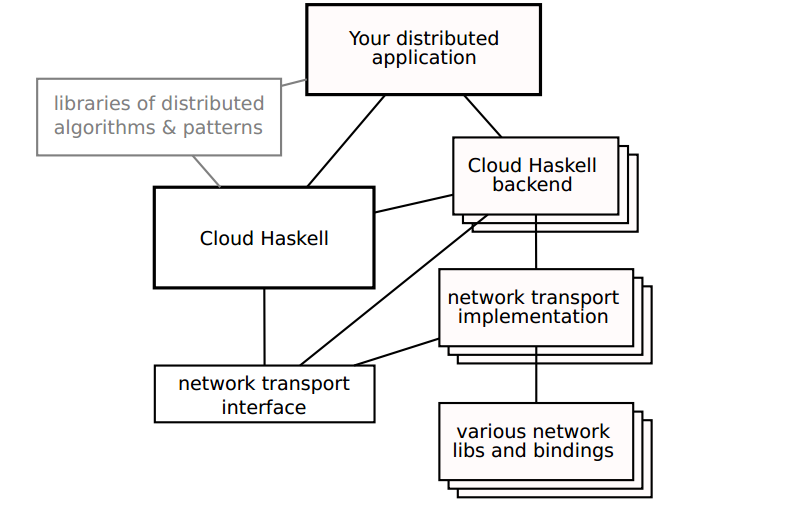
\includegraphics[scale=0.5]{design}

The architecture of Cloud Haskell is highly decoupled from the
transport backend. A major issue with Erlang is that it is difficult
to use in exotic network protocols like infiniband, CCI, etc. Cloud
Haskell has a unified Network Transport interface which provides a
uniform abstraction for a variety of actual network protocols. Porting
a Cloud Haskell program to another network protocol is as simple as
using the corresponding network transport implementation for the given
protocol.  Even the Cloud Haskell module is a stub API which simply
re-exports the actual Cloud Haskell backend API. This makes it very
easy to try out competing implementations of Cloud Haskell itself.

\subsection{The Actor Model and Cloud Haskell}

The dominant model of programming a distributed application running in
a cluster of nodes is via message-passing. MPI cite and Actor
Model cite are the popular models for message-passing. In actor
model, isolated (no shared memory) lightweight processes are the
smallest program primitives. These processes communicate only by
sending and receiving messages.

\subsection{Actor vs Thread}

Although, Actor is a concurrency abstraction similar to Thread, it has
subtle differences which makes it suitable in a distributed setting. A
comparison is listed in the table below.

Actor	Thread
can create more actors	can create more threads
can have private local state	can have private local state
has NO shared state (isolated from other actors!)	has limited shared state
communicates with other actors via asynchronous message passing	communicates with other threads via shared variables

The essential difference between the two is about isolation and
message passing. The appeal of actor model is its simplicity. By
avoiding shared state, it eliminates a whole class of concurrency bugs
by definition. It is easier to reason about because each actor can now
be reasoned about in isolation and independent of other actors.

More formally, an actor is a computational entity that, in response to a
message it receives, can concurrently :
\begin{itemize}
\item send a finite number of messages to other actors
\item create a finite number of new actors
\item designate the behavior to be used for the next message it receives
\end{itemize}

The only popular programming language based on actor model is Erlang.
Recently there has been a rise in the number of different
implementations of actor model. Instead of designing a new programming
language, the current actor based systems are implemented by embedding
as a concurrency paradigm inside a host language. This has obvious
advantages which are discussed in {cite}. Some popular
implementations are Akka (Scala and Java), Celluloid (Ruby) and Cloud
Haskell (Haskell).

\section{The Core API}

For complete documentation of Cloud Haskell API, the haddock
documentation can be read at {cite}.

The central abstraction in Cloud Haskell for message passing is the
Process monad. It keeps track of the state associated with a process,
primarily the message queue associated with the process. Any code
running in the Process monad has access to the data structures
representing the process and can pass these data structures to other
Process-monadic functions that it calls. All functions dealing with
sending and receiving of messages, spawning and linking processes must
be in the Process monad.

Since Process monad in an instance of MonadIO, arbitrary IO functions
can be called in Process monad via liftIO.

ProcessId is a type corresponding to the process identifier. NodeId is
similarly for nodes.

Any type which is an instance of Typeable and Binary is also an
instance of Serializable.

send takes a process-id and a serializable message and sends it
asynchronously to the corresponding process.
An example in the next section demonstrates the send and receive
functions.

\begin{program}

\caption[Cloud Haskell API]
{Core API}

\label{fig:cloud-haskell-api}
\begin{minted}{haskell}

instance Monad Process
instance MonadIO Process

data ProcessId
data NodeId

class (Typeable a, Binary a) => Serializable a

send :: Serializable a => ProcessId -> a -> Process ()
expect :: Serializable a => Process a

spawn :: NodeId -> Closure (Process ()) -> Process ProcessId

getSelfPid :: Process ProcessId
getSelfNode :: Process NodeId

\end{minted}
\end{program}


\section{Ping Pong in Cloud Haskell}

\begin{program}

\caption[Ping Pong in Cloud Haskell]
{Ping Pong in Cloud Haskell}

\label{fig:ping-pong-intro}
\begin{minted}{haskell}

module Main where
import Control.Concurrent ( threadDelay )
import Data.Binary
import Data.Typeable
import Control.Distributed.Process
import Control.Distributed.Process.Node
import Network.Transport.TCP

data Ping = Ping deriving (Typeable)
-- binary instance declaration of Ping
instance Binary Ping where
    put Ping = putWord8 0
    get      = do { getWord8; return Ping }
-- Ping is now serializable
server rPing = do
    Ping <- receiveChan rPing
    liftIO $ putStrLn "Got a ping!"

client :: SendPort Ping -> Process ()
client sPing =
    sendChan sPing Ping

ignition :: Process ()
ignition = do
    -- start the server
    sPing <- spawnChannelLocal server
    -- start the client
    spawnLocal $ client sPing
    liftIO $ threadDelay 100000 -- wait a while

main :: IO ()
main = do
    Right transport <- createTransport "127.0.0.1" "8080"
                            defaultTCPParameters
    node <- newLocalNode transport initRemoteTable
    runProcess node ignition

\end{minted}
\end{program}

This program is the hello world equivalent in distributed systems. A
client process sends a Ping to the server process. On receiving the
Ping, the server process prints a message ``Got a Ping''.

In main, we initialize a network transport tcp backend, setup a local
node and run the process ``ignition'' on the local node.

The process ``ignition'' spawn the ``server'' process and the
``client'' process on the local node and waits a while otherwise the
child processes will get killed when the parent terminates.

A channel is a tuple (SendPort a, ReceivePort a) on which only values
of type ``a'' can be transmitted. In this case, it is the data type
Ping. We create a binary instance of Ping to make it serializable.

The client sends Ping on the SendPort of server. In case of server,
receiveChan blocks until a message of type Ping is received on the
receive port. On receiving the message, server prints ``Got a Ping''
to the console.
\chapter{Related work}

The overall field concerning hot code reloading in software is called
Dynamic Software Updating (DSU). DSU is a field of research focused on
safely upgrading programs while they are running {cite}. Although
there is no existing research on DSU in the area of distributed
functional programming, there is lot of work in the field of
imperative and object oriented programming languages. We will briefly
describe the main ideas and concepts found in the literature. For a
detailed survey of DSU systems, {cite} is a very good resource.

\section{Formal specification of DSU}

Any running program can be thought of a tuple (\delta, P) . \delta is the
current program state and P is the current program code. DSU systems
transfer a running program (\delta, P) to (\delta', P'). The state
must be transformed into a representation P' expects. This requires a
state transformer function. Thus, DSU transforms (\delta, P) to
(S(\delta), P). An update is considered valid if and only if the
running program (S(\delta), P') can be reduced to a point tuple
(\delta, P') that is reachable from the starting point of the new
version of the program, ($\delta_{init}$, P').  For a formal
description of this ``validity'' , please refer to {cite}.

Although this is one formal definition for DSU, there is no consensus
on the standard definition of DSU applicable in all cases. {cite}
presents a list of definitions and requirements according to different
authors.

\section{Related ideas and techniques}

In this section, we briefly discuss the most relevant concepts and
techniques commonly used in the field of DSU systems.

\subsection{Quiescence}


\subsection{Binary Code Rewriting}

Some authors mostly in Java and C propose rewriting of the binary code of the programs in memory. Fraby was one of the fir 
\subsection{Proxies, Intermediaries and Indirection Levels}

\subsection{Intrusion and Cooperation}

\subsection{State Transfer}

\subsection{Transformation Functions}

\subsection{Using underlying facilities}

\subsection{Version Coexistence}


\section{DSU and Functional Programming}

\subsection{Haskell}

dons thesis
safecopy

\subsection{Erlang}


erlang's unspecified upgrade behaviour
Erlang requires no safety guarantees on updates cite.
haskell reloading facility by don;s thesis

% \input{applications}
% \chapter{Related work}

The overall field concerning hot code reloading in software is called
Dynamic Software Updating (DSU). DSU is a field of research focused on
safely upgrading programs while they are running {cite}. Although
there is no existing research on DSU in the area of distributed
functional programming, there is lot of work in the field of
imperative and object oriented programming languages. We will briefly
describe the main ideas and concepts found in the literature. For a
detailed survey of DSU systems, {cite} is a very good resource.

\section{Formal specification of DSU}

Any running program can be thought of a tuple (\delta, P) . \delta is the
current program state and P is the current program code. DSU systems
transfer a running program (\delta, P) to (\delta', P'). The state
must be transformed into a representation P' expects. This requires a
state transformer function. Thus, DSU transforms (\delta, P) to
(S(\delta), P). An update is considered valid if and only if the
running program (S(\delta), P') can be reduced to a point tuple
(\delta, P') that is reachable from the starting point of the new
version of the program, ($\delta_{init}$, P').  For a formal
description of this ``validity'' , please refer to {cite}.

Although this is one formal definition for DSU, there is no consensus
on the standard definition of DSU applicable in all cases. {cite}
presents a list of definitions and requirements according to different
authors.

\section{Related ideas and techniques}

In this section, we briefly discuss the most relevant concepts and
techniques commonly used in the field of DSU systems.

\subsection{Quiescence}


\subsection{Binary Code Rewriting}

Some authors mostly in Java and C propose rewriting of the binary code of the programs in memory. Fraby was one of the fir 
\subsection{Proxies, Intermediaries and Indirection Levels}

\subsection{Intrusion and Cooperation}

\subsection{State Transfer}

\subsection{Transformation Functions}

\subsection{Using underlying facilities}

\subsection{Version Coexistence}


\section{DSU and Functional Programming}

\subsection{Haskell}

dons thesis
safecopy

\subsection{Erlang}


erlang's unspecified upgrade behaviour
Erlang requires no safety guarantees on updates cite.
haskell reloading facility by don;s thesis

% \input{conclusions}

\begin{singlespace}
\cleardoublepage
\phantomsection \label{listoffig}
\addcontentsline{toc}{chapter}{References}
\renewcommand\bibname{References}
\printbibliography
\nocite{*}
\end{singlespace}


\end{document}
